%--------------------------------------------------------------------------------
%\documentclass{article}

\documentclass[a4paper, 12pt]{article}
\usepackage[T1]{fontenc} 
\usepackage[bf]{caption}
\usepackage{hyperref}
\usepackage[all]{hypcap}
\usepackage[utf8]{inputenc}
\usepackage{graphicx}
\usepackage[czech, english]{babel}
\selectlanguage{english}
\usepackage{subfig}                % \subfloat
\usepackage{color}
\usepackage{url}
\inputencoding{utf8}
%\usepackage[bf]{caption2}
\usepackage{hyperref}
\usepackage[all]{hypcap}
\hypersetup{colorlinks=false, linkbordercolor=1 1 1, citebordercolor=1 1 1}
\usepackage[right]{lineno}
\renewcommand\linenumberfont{\normalfont\tiny\color{blue}}


\title{Visualization of volumetric data}
\author{Boris Burkalo <xburka00@stud.fit.vutbr.cz>}
\date{\today}


%--------------------------------------------------------------------------------


\begin{document}
\selectlanguage{english}
\maketitle

\section{Introduction}
This project variant studies approaches to volumetric rendering and implements a volumetric renderer. This type of renderer is able to visualize volumetric
data as seemingly continuous 3D models. With these models then user can manipulate and visualize them in a way that is fitting to the use case
they pursue. Volumetric rendering is heavily used in medicine to visualize data from CT scans.

%%%%%%%%%%%%%%%%%%%%%%%%%%%%%%%%%%%%%%%%%%%%%%%%%%%%%%%%%%%%%%%%%%%%%%%%%%%%%%%%%%%%%%%%

\section{Theory}
This solution implements a single-pass volumetric raycasting as mentioned in \cite{gpu-accelerated-rendering-article}. 
This type of approach, as it has in the title, is able to render the whole scene in only one render pass and 
therefore is faster than the multi-pass approaches.

\subsection{Raycasting}
Raycasting is a form of visualizing volumetric data by casting a ray from camera position into the scene for each pixel and sampling the color along
the direction of the ray at given interval.
In practice it means that for each ray cast from position of the camera in the direction of a pixel, entry points and exit points are found. These two points
mark the points where the ray enters or exits the volume respectively. When these two points are known, it is fairly trivial to sample the color at 
given intervals and blend them together. \\

\begin{figure}[htb]
  \centering
  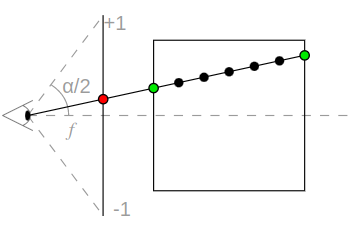
\includegraphics[width=6cm,keepaspectratio]{raycasting.png}
  \caption{Visualization of volumetric raycasting from \cite{gpu-accelerated-rendering-article}}
  \label{fig:raycasting}
\end{figure}

Two-pass volumetric raycasting is then performed, as the name suggests, in two passes. The first pass is used to find the entry and exit points
for each pixel of the viewport. These are then stored into two textures (Figure \ref{fig:textures} illustrates example of these two textures), 
which are used in the second pass. The second pass then takes care of the sampling and shading. This method however is not very efficient way 
of rendering volumetric data. \\

\begin{figure}[htb]
  \centering
  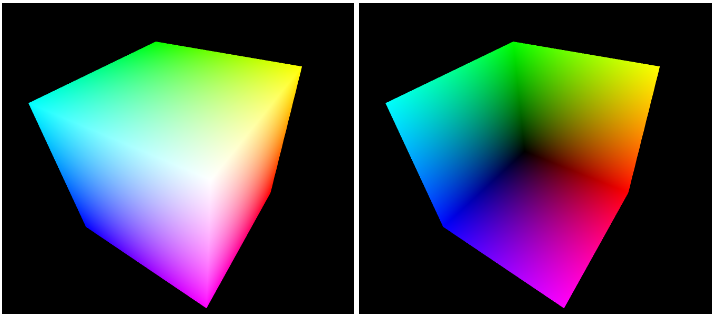
\includegraphics[width=8cm,keepaspectratio]{textures.png}
  \caption{Example of the entry and exit points textures from \cite{gpu-accelerated-rendering-article}}
  \label{fig:textures}
\end{figure}

Single-pass volumetric raycasting on the other hand offers a much better performance. In this approach the entry and exit points are computed in the
only render pass in the fragment shader by using the equation \ref{ray-equation}. In this equation $ \textbf{o} $ denotes the position of the camera and $ \textbf{v} $ denotes the
direction of the ray. The $ x $ and $ y $ components of $ \textbf{v} $ are the normalized device coordinates of the fragment, the $ z $ component is given
by focal length of the camera, which can be computed by equation \ref{focal-lenght}, where $ \alpha $ is the field of view of the camera.

\begin{equation}
  \label{ray-equation}
  \textbf{p} = \textbf{o} + t\textbf{v}
\end{equation}

\begin{equation}
  \label{focal-lenght}
  f = \frac{1}{\tan \frac{\alpha}{2}}
\end{equation}

With the knowledge of the equation \ref{ray-equation} the entry and exit points of the bounding box of the volume can be easily computed. Since the bounding box
of the volume is axis-aligned, the \textbf{SLAB} method mentioned in \cite{Shirley2021} or \cite{slab-method} is the obvious solution due to it's simpicity and speed. 
This method computes the ray-box intersections which then can be used to sample the color along the ray and visualize the volume.


%%%%%%%%%%%%%%%%%%%%%%%%%%%%%%%%%%%%%%%%%%%%%%%%%%%%%%%%%%%%%%%%%%%%%%%%%%%%%%%%%%%%%%%%

\section{Implementation details}
The solution is implemented in C++ programming language and uses modern OpenGL. For vector mathematics the GLM library has been used as it is efficient and very easy to use. \\
The solution is divided into a multitude of classes. The most notable one is class \texttt{VolumeTexture}, which encapsulates functionality of the 3D volumetric image represented
by 3D texture in OpenGL. This texture is then mapped onto the \texttt{UnitCube} object which represents the bounding box of the volume and is then in the fragment shader used for
computing the entry and exit points of the ray. \\
Another interesting class is the \texttt{TransferFunction} class. This class, based on voxel's intensity, gives the volume's voxel it's color which can be seen 
in the rendered image. The transfer function uses cubic spline to map the intensity in the input volumetric image to color and opacity in the output rendered image. At start of the application or if the
transfer function parameters are changed a 1D texture is generated in the \texttt{TransferFunction} class. This 1D texture represents how the intensities should be mapped to color and opacity.\\
The theory explained in previous chapter is then mostly implemented in the fragment shader, which is the perk of this single-pass approach. The fragment shader first assembles the
ray, then computes the entry and exit points of the volume's bounding box. With knowledge of this, it then samples intesity values of the volume represented by 3D texture, maps them
to color using the transfer function values stored in a 1D texture and blends them together. If the alpha value of the pixel's color is higher than 0.95, or the ray has exited the 
bounding box of the volume, the sampling is stopped, the color is tone-mapped and gamma-corrected and the fragment's color computation is finished. \\ 
\pagebreak

Classes in the \texttt{src/graphics} folder are used as an abstraction over actual OpenGL objects for easier manipulation and better code readability.


%%%%%%%%%%%%%%%%%%%%%%%%%%%%%%%%%%%%%%%%%%%%%%%%%%%%%%%%%%%%%%%%%%%%%%%%%%%%%%%%%%%%%%%%

\section{Evaluation}
This rather simple volumetric renderer is able to visualize smaller volumetric datasets (in units of tens of MBs) very well in real time on a device with integrated graphics card. 
However if performance would be a problem for the user, the sampling rate at which the volume is sampled along the ray, can be set to a smaller value, so the volume visualization can be faster.\\
The solution also allows to customize the visualization by implementing the transfer function functionality as mentioned in previous chapter. The transfer function control points can also be 
user-defined and set within the GUI itself. The solution also provides functionality for visualizing each individual frame of the volumetric dataset in X, Y and Z direction (see \ref{fig:surfaceplanes}). User can also 
take a screenshot of the created scene, which is saved to user's device. On top of that a quaternion arcball camera has been implemented for better inspection of the rendered volume. \\

\begin{figure}[htb]
  \centering
  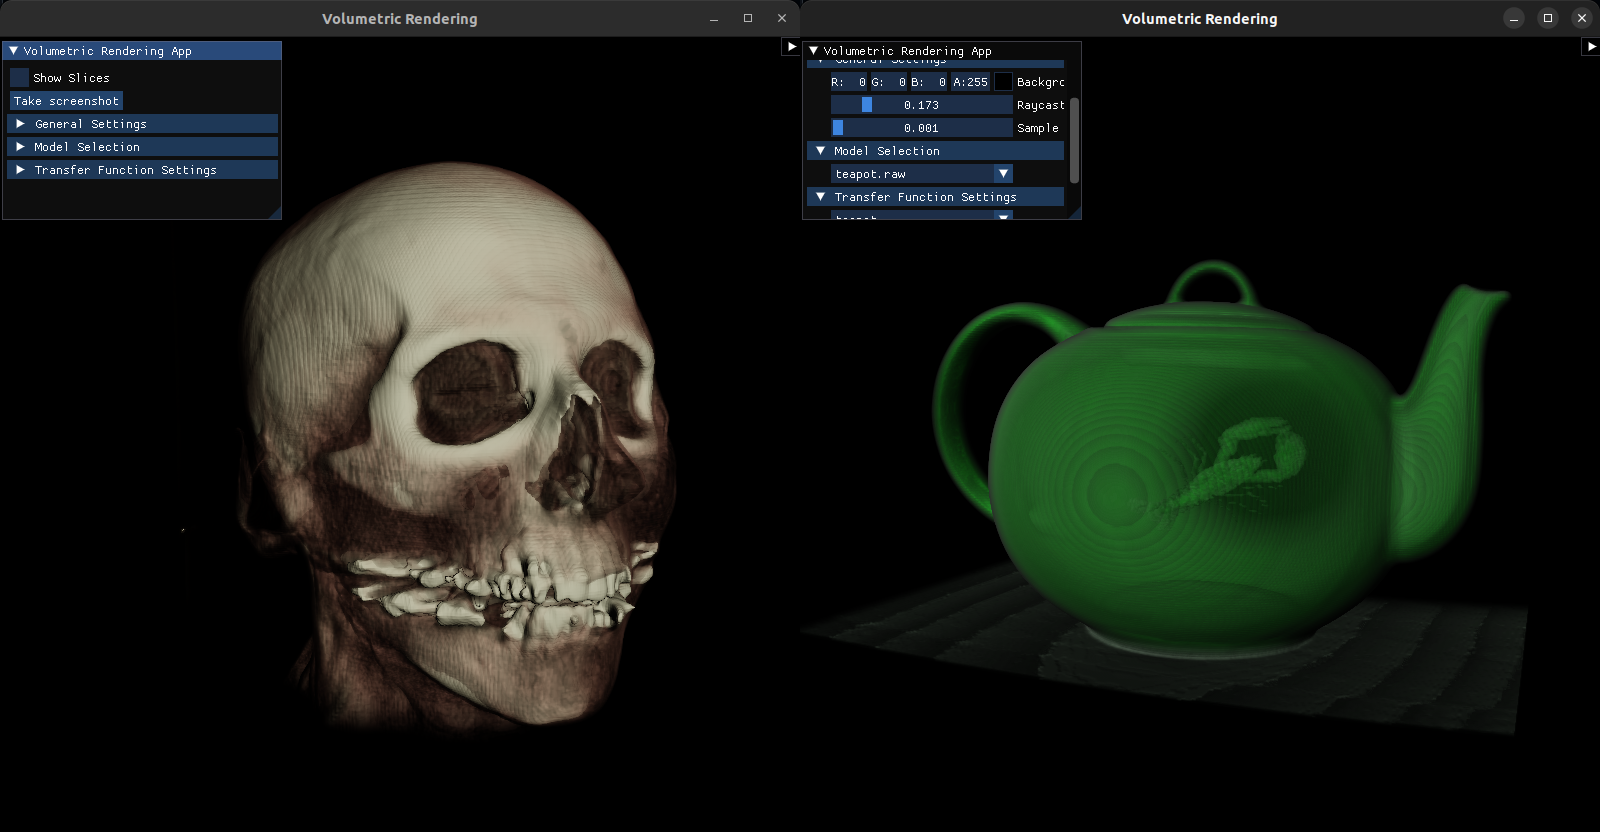
\includegraphics[width=14cm,keepaspectratio]{merged_sample1.png}
  \caption{Sample images taken from the project's solution.}
  \label{fig:textures}
\end{figure}

\begin{figure}[htb]
  \centering
  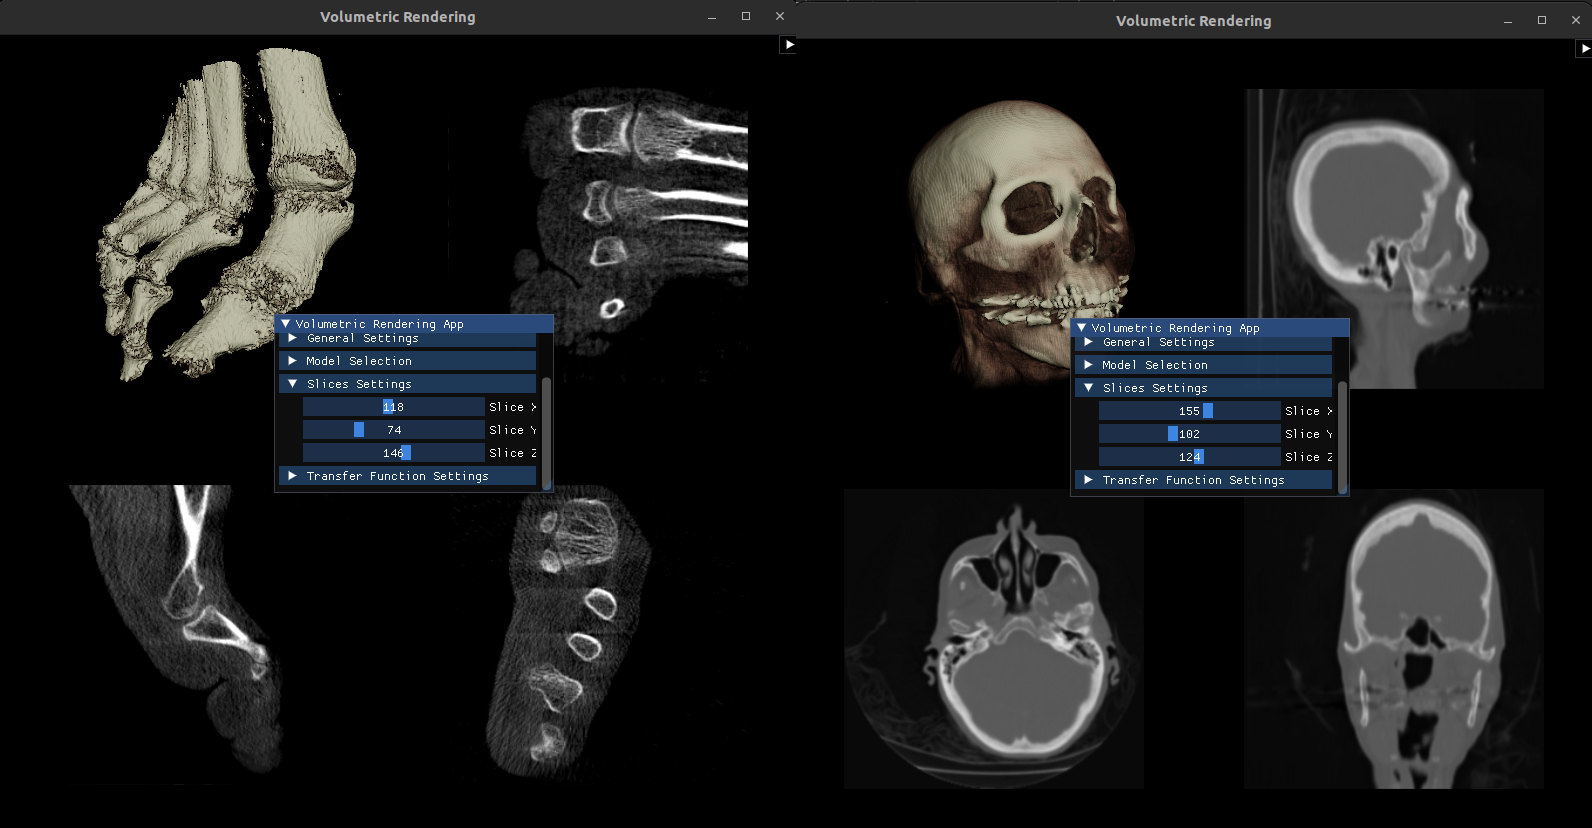
\includegraphics[width=14cm,keepaspectratio]{foot.png}
  \caption{Sample images taken from the project's solution.}
  \label{fig:surfaceplanes}
\end{figure}

\newpage
%%%%%%%%%%%%%%%%%%%%%%%%%%%%%%%%%%%%%%%%%%%%%%%%%%%%%%%%%%%%%%%%%%%%%%%%%%%%%%%%%%%%%%%%

\section{Conclusion}
Overall I'm happy with the solution I have implemented. The solution gives decent results in real-time and provides decent functionality for the user to play with. However of course
there are some things that still could be added. In the future I'd like to add some graph visualization of the transfer function settings, as in the state it is now, it can be a little confusing. 
I would also like to make the whole renderer a bit faster as it can get a bit slower in bigger windows on larger displays. I would also like to add functionality for visualizing various formats of
volumetric data such as DICOMs, because now the renderer visualizes only raw data with given dimensions.


\bibliographystyle{alpha}
\begin{flushleft}
  \bibliography{project}
\end{flushleft}

%\appendix
%\newpage
%\section{}

\end{document}
